\documentclass[unknownkeysallowed]{beamer}
\usepackage[french,english]{babel}
\usepackage{../sty/beamer_js}
\usepackage{../sty/shortcuts_js}

\addbibresource{../biblio/references_all.bib}

\begin{document}


%%%%%%%%%%%%%%%%%%%%%%%%%%%%%%%%%%%%%%%%%%%%%%%%%%%%%%%%%%%%%%%%%%%%%%%%%%%%%%%
%%%%%%%%%%%%%%%%%%%%%%             Headers               %%%%%%%%%%%%%%%%%%%%%%
%%%%%%%%%%%%%%%%%%%%%%%%%%%%%%%%%%%%%%%%%%%%%%%%%%%%%%%%%%%%%%%%%%%%%%%%%%%%%%%



%%%%%%%%%%%%%%%%%%%%%%%%%%%%%%%%%%%%%%%%%%%%%%%%%%%%%%%%%%%%%%%%%%%%%%%%%%%%%%%
\begin{frame}
\bigskip
\bigskip
\begin{center}{
\LARGE\color{marron}
\textbf{Noisy and Missing Data Regression: Distribution-Oblivious Support Recovery}
\textbf{ }\\
\vspace{0.5cm}
}

\color{marron}
\textbf{}
\end{center}

\vspace{0.5cm}

\begin{center}
\textbf{Rudolf Römisch} \\
\vspace{0.1cm}
\vspace{0.5cm}
Université de Montpellier \\
\end{center}

\centering
\includegraphics[width=0.13\textwidth]{Logo}

\end{frame}
%%%%%%%%%%%%%%%%%%%%%%%%%%%%%%%%%%%%%%%%%%%%%%%%%%%%%%%%%%%%%%%%%%%%%%%%%%%%%%%



%%%%%%%%%%%%%%%%%%%%%%%%%%%%%%%%%%%%%%%%%%%%%%%%%%%%%%%%%%%%%%%%%%%%%%%%%%%%%%%
%%%%%%%%%%%%%%%%%%%%%%%%       PLAN      %%%%%%%%%%%%%%%%%%%%%%%%%%%%%%%%%%%%%%
%%%%%%%%%%%%%%%%%%%%%%%%%%%%%%%%%%%%%%%%%%%%%%%%%%%%%%%%%%%%%%%%%%%%%%%%%%%%%%%



%%%%%%%%%%%%%%%%%%%%%%%%%%%%%%%%%%%%%%%%%%%%%%%%%%%%%%%%%%%%%%%%%%%%%%%%%%%%%%%
\begin{frame}{Table of Contents}
\tableofcontents[hideallsubsections]
\end{frame}


%%%%%%%%%%%%%%%%%%%%%%%%%%%%%%%%%%%%%%%%%%%%%%%%%%%%%%%%%%%%%%%%%%%%%%%%%%%%%%%
%%%%%%%%%%%%%%%%%%%%%%%%%%%%%%%%%%%%%%%%%%%%%%%%%%%%%%%%%%%%%%%%%%%%%%%%%%%%%%%
\section{Introduction}
\label{sec:introdcution}
%%%%%%%%%%%%%%%%%%%%%%%%%%%%%%%%%%%%%%%%%%%%%%%%%%%%%%%%%%%%%%%%%%%%%%%%%%%%%%
%%%%%%%%%%%%%%%%%%%%%%%%%%%%%%%%%%%%%%%%%%%%%%%%%%%%%%%%%%%%%%%%%%%%%%%%%%%%%%%
\begin{frame}{Situation}
	\begin{itemize}
		\item Typical: Regression with known covariates and without noise
		\item But: For high-dimension it is not the case
		\item Goal: Algorithm which recovers support
	\end{itemize}
\end{frame}
%%%%%%%%%%%%%%%%%%%%%%%%%%%%%%%%%%%%%%%%%%%%%%%%%%%%%%%%%%%%%%%%%%%%%%%%%%%%%%%
%%%%%%%%%%%%%%%%%%%%%%%%%%%%%%%%%%%%%%%%%%%%%%%
\subsection{Contributions}

\begin{frame}{Contributions}
	\begin{itemize}
		\item OMP and Support Recovery
		\item $l^2$-bounds
		\item Numerical Simulations
		\item Obtaining Bounds on OMP Performing
	\end{itemize}
\end{frame}


%%%%%%%%%%%%%%%%%%%%%%%%%%%%%%%%%%%%%%%%%%%%%%%%%%%%%%%%%%%%%%%%%%%%%%%%%%%%%%%
\subsection{A second example}
\label{sub:deuxiem_exmple}
%%%%%%%%%%%%%%%%%%%%%%%%%%%%%%%%%%%%%%%%%%%%%%%%%%%%%%%%%%%%%%%%%%%%%%%%%%%%%%%
\section{Problem Setup}
\begin{frame}{Linear Model}
	\begin{equation*}
	y_i = \langle x_i,\beta^*\rangle + e_i, \quad	i=1,...,n
	\end{equation*}\ \\
	We have two different cases:
	\begin{itemize}
		\item[1.] Covariates with additive Noise
		\item[2.] Covariates with Missing Data
	\end{itemize}
\end{frame}

\begin{frame}{Sub-Gaussian Model}
	\begin{definition}
		Sub-Gaussian Matrix: A zero-mean matrix V is called sub-Gaussian with parameter $(\frac{1}{n}\Sigma,\frac{1}{n}\sigma^2)$ if (a) Each row $v_i^T \in \mathbb{R}^p$ of V is sampled independently and has $\mathbb{E}[v_iv_i^T]=\frac{1}{n}\Sigma$. (b) For any unit vector $u \in \mathbb{R}^p$, $u^Tv_i$ is a sub-Gaussian random variable with parameter at most $\frac{1}{\sqrt{n}}\sigma$.
	\end{definition}
	\begin{definition}
		Sub-Gaussian Design Model: We assume X, W and e are sub-Gaussian with parameters $(\frac{1}{n}\Sigma_x,\frac{1}{n})$, $(\frac{1}{n}\Sigma_w, \frac{1}{n}\sigma_w)$ and $(\frac{1}{n}\sigma_e^2, \frac{1}{n}\sigma_e^2)$, respectively, and are independent of each other. For the case of independence across columns we call this the $Independent$ sub-Gaussian Model.
	\end{definition}
\end{frame}



\section{Distribution-Oblivious Support Recovery via Orthogonal Matching Pursuit}
\begin{frame}{Support Identifcation}
	\begin{theorem}
		Under the Independent sub-Gaussian Design model and Additive Noise model, supp-OMP identifies the correct support of $\beta^*$ with high probability, provided
		\begin{equation*}
		n \gtrsim (1+\sigma^2_w)^2klog(p),
		\end{equation*}
		\begin{equation*}
		|\beta^*_i| \geq 16(\sigma_w||\beta^*||_2 + \sigma_e)\sqrt{\frac{log(p)}{n}},
		\end{equation*}
		for all $i \in supp(\beta^*)$.
	\end{theorem}

\end{frame}


\begin{frame}{Support Identifcation}
	\begin{theorem}
		Let $\sigma^2_z = \sigma^2_x + \sigma^2_w$. Under the independent Gaussian model where the covariance of X, W and e are isotropic, if 
		\begin{align*}
		n &\lesssim (\sigma^2_w + \frac{\sigma^2_z \sigma^2_e}{R^2})k log(\frac{p}{k}) \quad or\\
		b_{min} &\lesssim \sqrt{(\sigma^2_w R^2 + \sigma^2_z \sigma^2_e) \frac{log(p/k)}{n}}, \quad then\\
		\mathcal{M}_0 &\geq 1.
		\end{align*}
	\end{theorem}

\end{frame}

\begin{frame}{Estimating the Non-Zero Coeffcients}
	\begin{theorem}
		Under the Independent sub-Gaussian Design model and Additive Noise model, the output of our estimator satisfies:
		\begin{itemize}
			\item (Knowledge of $\Sigma_w$): $||\hat{\beta} - \beta^*||_2 \lesssim [(\sigma_w + \sigma_w^2)||\beta^*||_2 + \sigma_e \sqrt{1+\sigma_w^2}]\sqrt{\frac{klog(p)}{n}}$.
			\item (Knowledge of $\Sigma_x$): $||\hat{\beta} - \beta^*||_2 \lesssim [(1 + \sigma_w)||\beta^*||_2 + \sigma_e \sqrt{1+\sigma_w^2}]\sqrt{\frac{klog(p)}{n}}$.
		\end{itemize}
	\end{theorem}
\begin{theorem}
	Let $\sigma_z^2 = \sigma_x^2 + \sigma_w^2$, and suppose $8 \geq k \geq p/2$ and $n \lesssim k log (p/k)$. Under the independent Gaussian model where the covariance of X, W and e are isotropic, the $l^2$-error is bounded below: $M_2 \gtrsim \sqrt{(\sigma_w^2 R^2 + \sigma_z^2 \sigma_e^2)\frac{k}{n} log(\frac{p}{k})}$.
\end{theorem}
\end{frame}


\begin{frame}{Missing Data}
	\begin{theorem}
		Under the Independent sub-Gaussian Design model and missing data model, supp-OMP identifies the correct support of $\beta^*$ provided
		\begin{align*}
		n &\gtrsim \frac{1}{(1-\rho)^4}k log(p),\\
		|\beta^*_i| &\geq \frac{16}{1-\rho}(||\beta^*||_2 + \sigma_e) \sqrt{\frac{log(p)}{n}},
		\end{align*}
		for all $i \in supp(\beta^*)$. Moreover; the output of estimator (2) with knowledge of $\rho$ satisfies
		\begin{equation*}
		||\hat{\beta} - \beta^*||_2 \lesssim (\frac{1}{(1-\rho)^2}||\beta^*||_2 + \frac{1}{1-\rho}\sigma_e)\sqrt{\frac{k log(p)}{n}}.
		\end{equation*}
	\end{theorem}
	
\end{frame}


\section{Numerical Simulations}
\begin{frame}{Additive Noise}
	\centering
	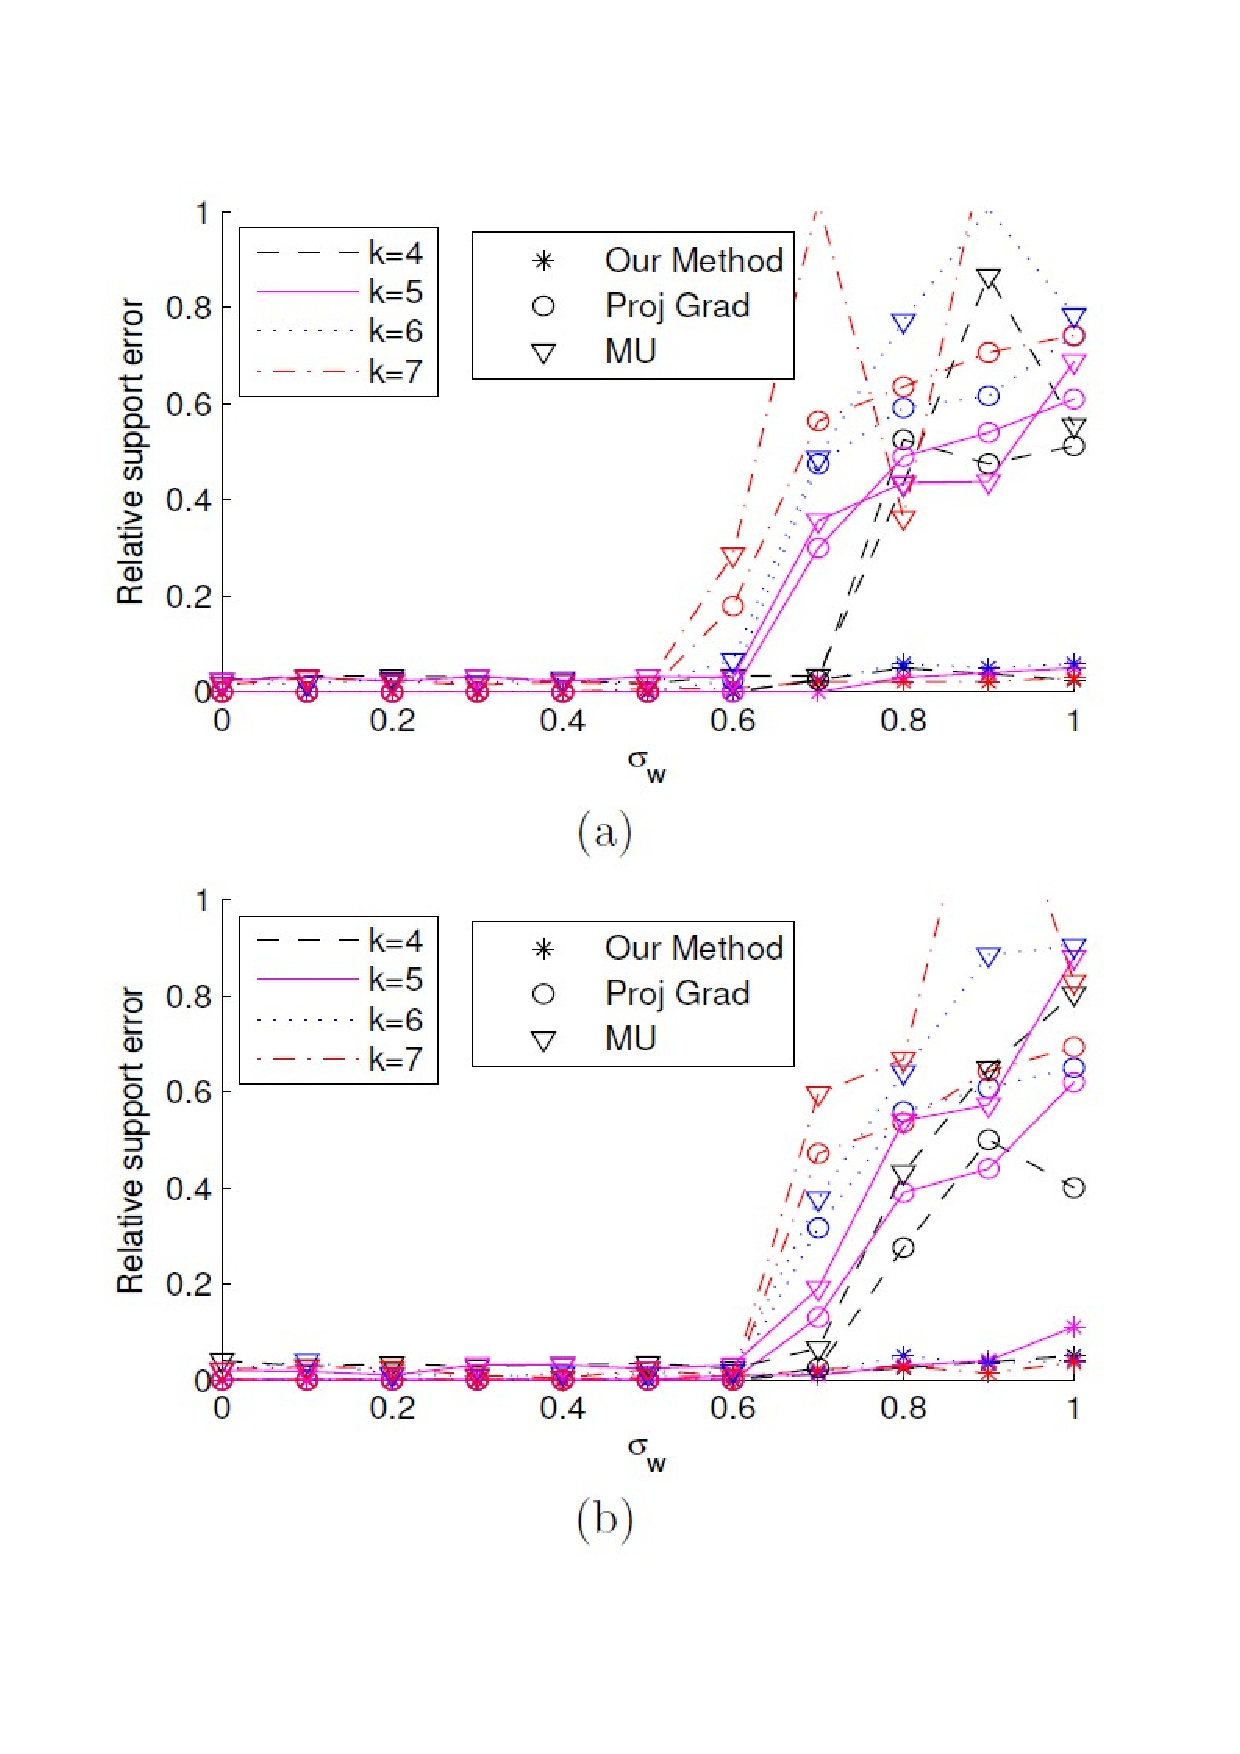
\includegraphics[scale=0.32]{relative_support_error.pdf}
\end{frame}
\begin{frame}{Missing Data}
	\centering
	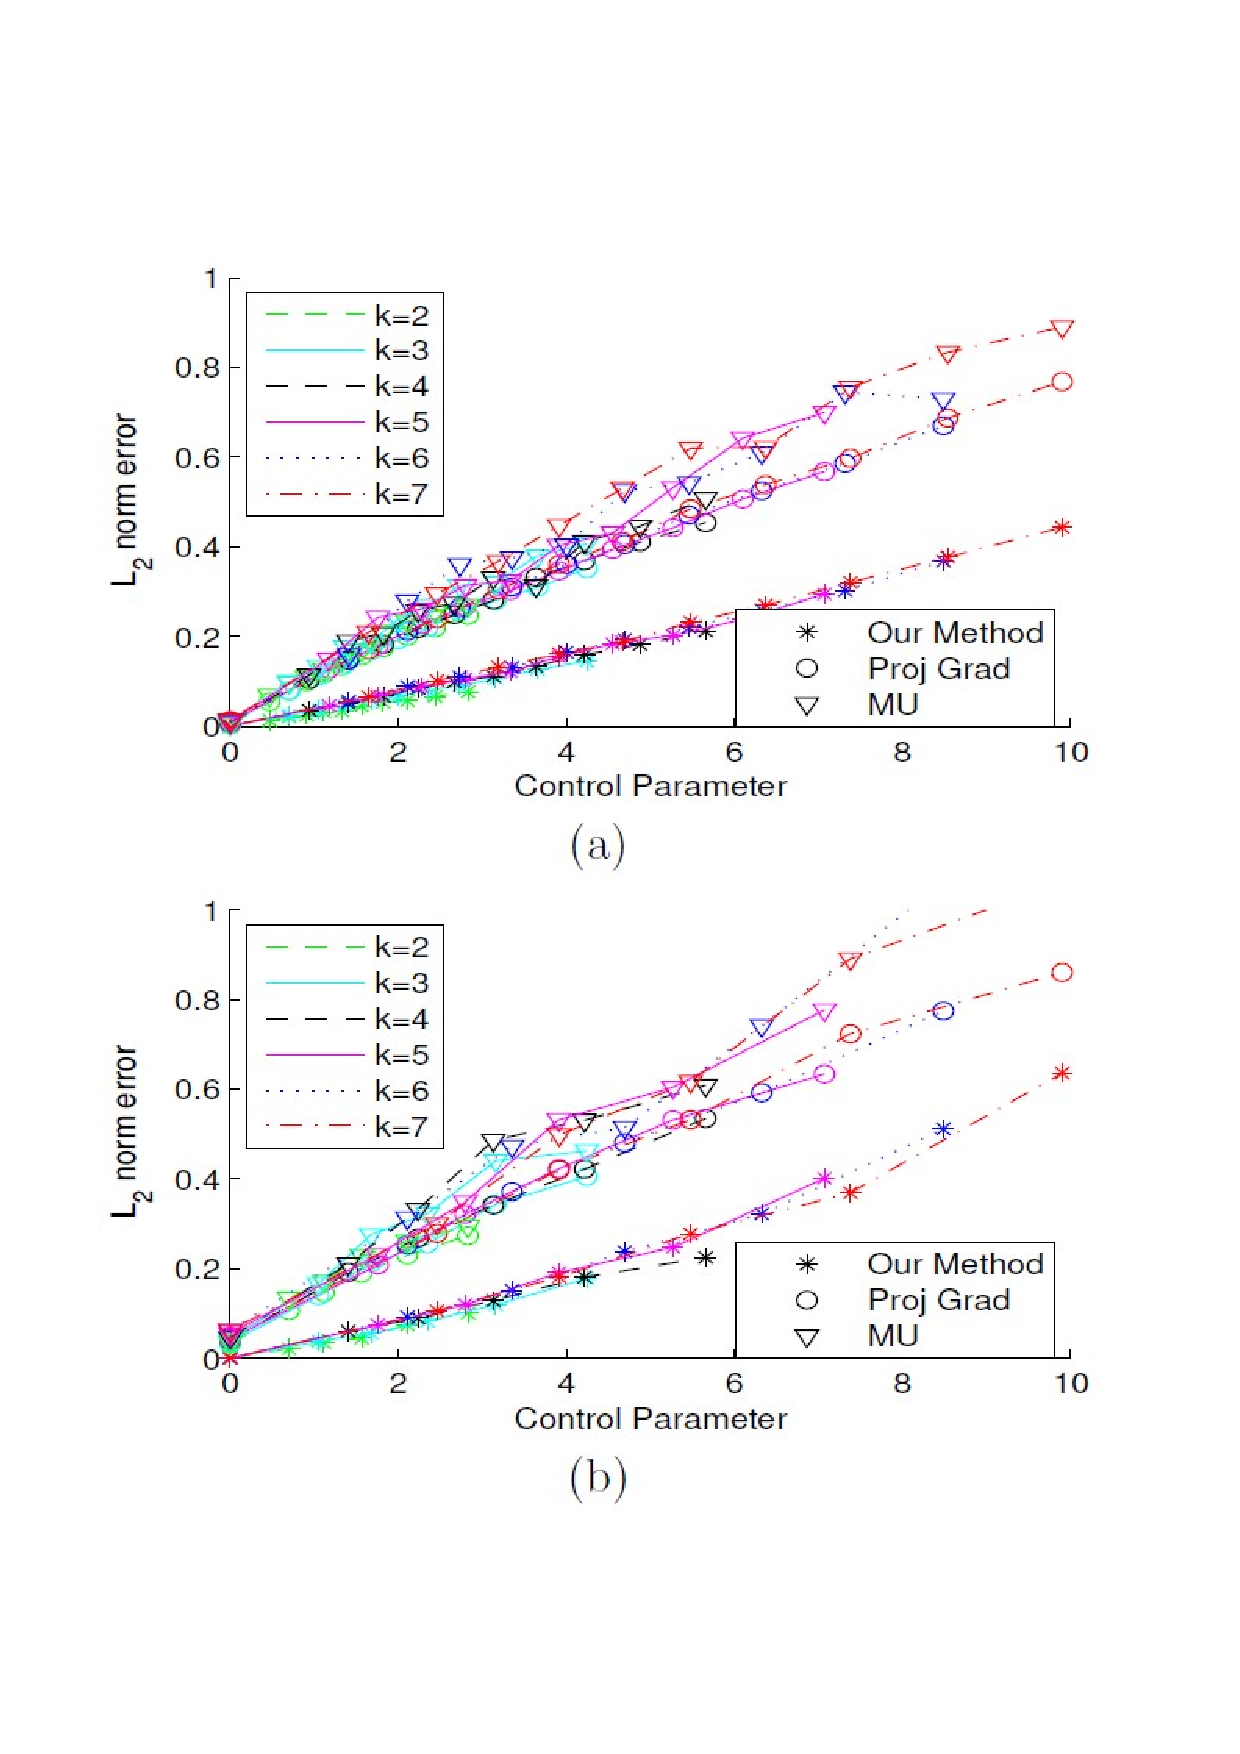
\includegraphics[scale=0.32]{l1_norm_error.pdf}
\end{frame}
%%%%%%%%%%%%%%%%%%%%%%%%%%%%%%%%%%%%%%%%%%%%%%%%%%%%%%%%%%%%%%%%%%%%%%%%%%%%%%%
%%%%%%%%%%%%%%%%%%%%%%%%%%%%%%%%%%%%%%%%%%%%%%%%%%%%%%%%%%%%%%%%%%%%%%%%%%%%%%%
\section{Conclusion}
\label{sec:conclusion}
%%%%%%%%%%%%%%%%%%%%%%%%%%%%%%%%%%%%%%%%%%%%%%%%%%%%%%%%%%%%%%%%%%%%%%%%%%%%%%%
%%%%%%%%%%%%%%%%%%%%%%%%%%%%%%%%%%%%%%%%%%%%%%%%%%%%%%%%%%%%%%%%%%%%%%%%%%%%%%%




%%%%%%%%%%%%%%%%%%%%%%%%%%%%%%%%%%%%%%%%%%%%%%%%%%%%%%%%%%%%%%%%%%%%%%%%%%%%%%%
\subsection{Rapidement}
\label{sub:rapidement}
%%%%%%%%%%%%%%%%%%%%%%%%%%%%%%%%%%%%%%%%%%%%%%%%%%%%%%%%%%%%%%%%%%%%%%%%%%%%%%%




 %%%%%%%%%%%%%%%%%%%%%%%%%%%%%%%%%%%%%%%%%%%%%%%%%%%%%%%%%%%%%%%%%%%%%%%%%%%%%%



\end{document}
